\documentclass[10 pt,usenames,dvipsnames, oneside]{article}
\usepackage{../../../modelo-ensino-medio}



\begin{document}

\begin{center}
  \begin{minipage}[l]{3cm}

\includegraphics[width=2cm]{logo}    
\end{minipage}\hfill
\begin{minipage}[r]{.8\textwidth}
 {\Large \scshape Atividade: Trajetória de uma bola de futebol}  
\end{minipage}
\end{center}
\vspace{.2cm}

\ifdefined\prof
%Habilidades da BNCC
% \begin{objetivos}
% \item 
% \end{objetivos}

%Caixa do Para o Professor
\begin{goals}
%Objetivos específicos
\begin{enumerate}
\item Aplicar um sistema linear em contexto de modelagem de trajetória.
\end{enumerate}

\tcblower

%Orientações e sugestões
Professor, o item \titem{c)} dessa atividade é uma excelente oportunidade para que se trabalhe com os alunos a determinação das coordenadas do vértice de uma parábola não pelas fórmulas clássicas ($(x_v,y_v)=(\frac{-b}{2a}, \frac{-\Delta}{4a})$), mas observando a simetria da parábola em relação a uma reta perpendicular ao eixo $0x$ passando pelo vértice, portanto, pode-se obter $x_v$ como sendo o ponto médio entre as raízes e o $y_v=f(x_v)$. 

\end{goals}

\bigskip
\begin{center}
{\large \scshape Atividade}
\end{center}
\fi

\begin{figure}[H]
\centering
\noindent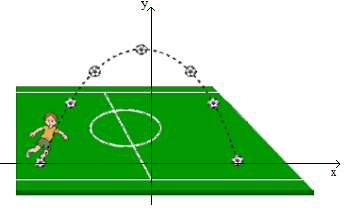
\includegraphics[width=325bp]{fadonelinho}
\caption{Adaptado de: \href{https://profes.com.br/felipes.rocha/blog/lancamento-obliquo-e-o-futebol}{Profes}}
\end{figure}

Após ver o vídeo em que Nelinho chuta a bola para fora do estádio, Mateus ficou fã do jogador e está praticando chutes altos com sua bola de futebol no campinho que há nas proximidades de sua casa. Mateus dá um chute na bola, que segue a trajetória de uma parábola. Considere que, numa visão frontal, considerou-se um sistema de coordenadas cartesianas como o da figura, onde o eixo $x$ é paralelo à linha lateral do campo e o eixo $y$ é perpendicular ao plano do campo. Ao longo da trajetória, a bola parte do ponto $(-5,0)$, passa pelo ponto $(-2.5, 5)$ e toca o solo no ponto $(2.5, 0)$. Considere a função quadrática $f(x) = ax²+bx+c$ que modela a trajetória da bola.

\begin{enumerate}
\item{}
Utilizando as informações sobre os pontos do sistema de coordenadas informados no enunciado pelos quais a bola passa no decorrer do movimento, obtenha um sistema de 3 equações nas 3 incógnitas $a$, $b$ e $c$.

\item{}
Escalone e resolva o sistema do item \titem{a)};

\item{}
Determine a altura máxima atingida pela bola após o chute dado por Mateus.

\end{enumerate}

\ifdefined\prof
\begin{solucao}

\begin{enumerate}
\item 
$
\left \{
\begin{aligned}
25a-5b+c&=0\\
6{,}25a-2{,}5b+c&=5\\
6{,}25a+2{,}5b+c&=0
\end{aligned}
\right.
$
\item $(a,b,c)=(-\dfrac{2}{5},-1,5)$.
\item $5{,}625$m.
\end{enumerate}

\end{solucao}
\fi

\end{document}